%%%%%%%%%%%%%%%%%%%%%%%%%%%%%%%%%%%%%%%%%
% Programming/Coding Assignment
% LaTeX Template
%
% This template has been downloaded from:
% http://www.latextemplates.com
%
% Original author:
% Ted Pavlic (http://www.tedpavlic.com)
%
% Note:
% The \lipsum[#] commands throughout this template generate dummy text
% to fill the template out. These commands should all be removed when 
% writing assignment content.
%
% This template uses a Perl script as an example snippet of code, most other
% languages are also usable. Configure them in the "CODE INCLUSION 
% CONFIGURATION" section.
%
%%%%%%%%%%%%%%%%%%%%%%%%%%%%%%%%%%%%%%%%%

%%%%%%%%%%%%%%%%%%%%%%%%%%%%%%%%%%%%%%%%%%%%%%
% Modified by George Z. Zachos
% on March 28, 2017 for the Parallel Systems
% and Programming course @cse.uoi.gr
%%%%%%%%%%%%%%%%%%%%%%%%%%%%%%%%%%%%%%%%%%%%%%

%----------------------------------------------------------------------------------------
%	PACKAGES AND OTHER DOCUMENT CONFIGURATIONS
%----------------------------------------------------------------------------------------

\documentclass{article}

\usepackage{fancyhdr} % Required for custom headers
\usepackage{lastpage} % Required to determine the last page for the footer
\usepackage{extramarks} % Required for headers and footers
\usepackage[usenames,dvipsnames]{xcolor} % Required for custom colors
\usepackage{graphicx} % Required to insert images
\usepackage{listings} % Required for insertion of code
\usepackage{courier} % Required for the courier font
% Margins
\topmargin=-0.45in
\evensidemargin=0in
\oddsidemargin=0in
\textwidth=6.5in
\textheight=9.0in
\headsep=0.25in

\linespread{1.1} % Line spacing

% Set up the header and footer
\pagestyle{fancy}
\lhead{\hmwkAuthorName} % Top left header
\chead{\hmwkClass: \hmwkTitle} % Top center head
\rhead{\firstxmark} % Top right header
\lfoot{\lastxmark} % Bottom left footer
\cfoot{} % Bottom center footer
\rfoot{Page\ \thepage\ of\ \protect\pageref{LastPage}} % Bottom right footer
\renewcommand\headrulewidth{0.4pt} % Size of the header rule
\renewcommand\footrulewidth{0.4pt} % Size of the footer rule

%\setlength\parindent{0pt} % Removes all indentation from paragraphs

%----------------------------------------------------------------------------------------
%	CODE INCLUSION CONFIGURATION
%----------------------------------------------------------------------------------------

\definecolor{MyDarkGreen}{rgb}{0.0,0.4,0.0} % This is the color used for comments
\lstloadlanguages{C}
\lstset{language=C,
        frame=single, % Single frame around code
        basicstyle=\small\ttfamily, % Use small true type font
        commentstyle=\usefont{T1}{pcr}{m}{sl}\color{MyDarkGreen}\small, % Comments small dark green courier font
        stringstyle=\color{Purple}, % Strings are purple
        showstringspaces=false, % Don't put marks in string spaces
        tabsize=5, % 5 spaces per tab
        morecomment=[l][\color{Blue}]{...}, % Line continuation (...) like blue comment
        numbers=left, % Line numbers on left
        firstnumber=0, % Line numbers start with line 0
        numberstyle=\tiny\color{Blue}, % Line numbers are blue and small
        stepnumber=1 % Line numbers go in steps of 1
}

% Creates a new command to include a perl script, the first parameter is the filename of the script (without .pl), the second parameter is the caption
\newcommand{\cscript}[2]{
\begin{itemize}
\item[]\lstinputlisting[caption=#2,label=#1]{#1.py}
\end{itemize}
}

\def\code#1{\texttt{#1}}
%----------------------------------------------------------------------------------------
%	DOCUMENT STRUCTURE COMMANDS
%	Skip this unless you know what you're doing
%----------------------------------------------------------------------------------------

% Header and footer for when a page split occurs within a problem environment
\newcommand{\enterProblemHeader}[1]{
\nobreak\extramarks{#1}{#1 continued on next page\ldots}\nobreak
\nobreak\extramarks{#1 (continued)}{#1 continued on next page\ldots}\nobreak
}

% Header and footer for when a page split occurs between problem environments
\newcommand{\exitProblemHeader}[1]{
\nobreak\extramarks{#1 (continued)}{#1 continued on next page\ldots}\nobreak
\nobreak\extramarks{#1}{}\nobreak
}

\setcounter{secnumdepth}{0} % Removes default section numbers
\newcounter{homeworkProblemCounter} % Creates a counter to keep track of the number of problems

\newcommand{\homeworkProblemName}{}
\newenvironment{homeworkProblem}[1][Problem \arabic{homeworkProblemCounter}]{ % Makes a new environment called homeworkProblem which takes 1 argument (custom name) but the default is "Problem #"
\stepcounter{homeworkProblemCounter} % Increase counter for number of problems
\renewcommand{\homeworkProblemName}{#1} % Assign \homeworkProblemName the name of the problem
\section{\homeworkProblemName} % Make a section in the document with the custom problem count
\enterProblemHeader{\homeworkProblemName} % Header and footer within the environment
}{
\exitProblemHeader{\homeworkProblemName} % Header and footer after the environment
}

\newcommand{\problemAnswer}[1]{ % Defines the problem answer command with the content as the only argument
\noindent\framebox[\columnwidth][c]{\begin{minipage}{0.98\columnwidth}#1\end{minipage}} % Makes the box around the problem answer and puts the content inside
}

\newcommand{\homeworkSectionName}{}
\newenvironment{homeworkSection}[1]{ % New environment for sections within homework problems, takes 1 argument - the name of the section
\renewcommand{\homeworkSectionName}{#1} % Assign \homeworkSectionName to the name of the section from the environment argument
\subsection{\homeworkSectionName} % Make a subsection with the custom name of the subsection
\enterProblemHeader{\homeworkProblemName\ [\homeworkSectionName]} % Header and footer within the environment
}{
\enterProblemHeader{\homeworkProblemName} % Header and footer after the environment
}

%----------------------------------------------------------------------------------------
%	NAME AND CLASS SECTION
%----------------------------------------------------------------------------------------

\newcommand{\hmwkTitle}{Homework \#1} % Assignment title
\newcommand{\hmwkDueDate}{Monday,\ April\ 7,\ 2017} % Due date
\newcommand{\hmwkClass}{MYE023} % Course/class
\newcommand{\hmwkClassTime}{} % Class/lecture time
\newcommand{\hmwkClassInstructor}{Vassilios V. Dimakopoulos} % Teacher/lecturer
\newcommand{\hmwkAuthorName}{George Z. Zachos} % Your name

%----------------------------------------------------------------------------------------
%	TITLE PAGE
%----------------------------------------------------------------------------------------

\title{
\vspace{2in}
\textmd{\textbf{\hmwkClass:\ \hmwkTitle}}\\
\normalsize\vspace{0.1in}\small{Due\ on\ \hmwkDueDate}\\
\vspace{0.1in}\large{\textit{\hmwkClassInstructor}}
\vspace{3in}
}

\author{\textbf{\hmwkAuthorName}}
\date{March 28, 2017} % Insert date here if you want it to appear below your name

%----------------------------------------------------------------------------------------

\setcounter{secnumdepth}{3}

\begin{document}

\maketitle

%----------------------------------------------------------------------------------------
%	TABLE OF CONTENTS
%----------------------------------------------------------------------------------------

\newpage
\tableofcontents
\newpage

%----------------------------------------------------------------------------------------
%	Exercise #1
%----------------------------------------------------------------------------------------

\section{Exercise \#1}
\subsection{About}
This exercise is about the calculation of the mathematical constant $\pi$ using \texttt{POSIX}
threads and dynamic scheduling. During dynamic scheduling the parallelizable loops are divided
into chunks of iterations (tasks) and are dispatched to the threads available to the runtime
system for execution. The dispatch takes place in respect to the current processor workload
where the thread executes and as a result load balancing is achieved. In case chunk size is
one ($1$) iteration, we refer to this technique as self-scheduling. The purpose of this
exercise is to time the calculation of $\pi$ and observe how altering the number of threads
will affect execution time for a given chunk size.

\subsection{Experiment details}

The calculation consists of $5*10^8$ loop iterations, while thread number takes value in \{1, 4, 16\} and
chunk size in \{1, 10, $10^2$, $10^3$, $10^4$, $10^5$\}.

\subsubsection{System Specifications}
The experiments were conducted on a Dell OptiPlex 7020:
\begin{itemize}
 \item CPU: Intel\textregistered \ Core\texttrademark \ i5-4590 CPU @ 3.30GHz (64 bit)
 \item RAM: 2 DIMMs x4GiB @ 1600MHz DDR3
 \item Cache line size: 64B (in all levels)
 \item Cache associativity:
 \begin{itemize}
  \item L1, L2: 8-way set associative
  \item L3: 12-way set associative
 \end{itemize}
\end{itemize}

\begin{figure}[htbp]
  \centering
  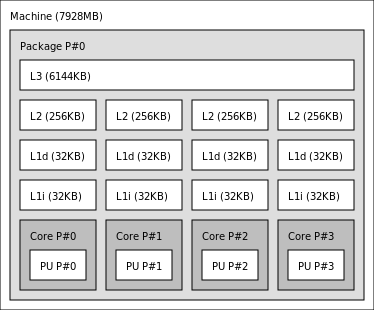
\includegraphics[width=0.5\columnwidth]{./opti7020-topo.png}
  \caption{Topology information of a Dell OptiPlex 7020}
\end{figure}

\pagebreak

\subsection{Timing Results}

In the following tables and plots the recorded execution times are displayed.

%------------------------------------ 1

\begin{table}[htbp]
  \centering
    \begin{tabular}{|c c||l l l l| l|} 
    \hline
    \multicolumn{7}{|c|}{Timing results of $\pi$ calculation (Time unit: seconds)} \\
    \hline
    Chunk Size & \# of threads & 1st run & 2nd run & 3rd run & 4thr run & Average time\\ [0.5ex] 
    \hline\hline
    1 & 1 & 18.451202 & 18.443870 & 18.444319 & 18.441278 & 18.44516725 \\ 
    \hline
    1 & 4 & 98.559317 & 98.393137 & 99.515415 & 98.189223 & 98.664273 \\
    \hline
    1 & 16 & 95.482310 & 95.205719 & 95.275233 & 95.197046 & 95.290077 \\ [1ex]
    \hline
    \end{tabular}
  \caption{Timing results of $\pi$ calculation using chunk size = 1 iteration}
\end{table}


\begin{figure}[htbp]
  \centering
  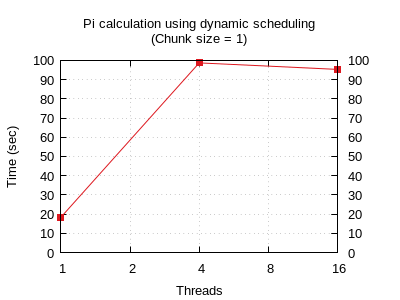
\includegraphics[width=0.55\columnwidth]{../ex1/plots/pi_c1.png}
  \caption{Timing results of $\pi$ calculation using chunk size = 1 iteration}
\end{figure}

%------------------------------------ 2

\begin{table}[htbp]
  \centering
    \begin{tabular}{|c c||l l l l| l|} 
    \hline
    \multicolumn{7}{|c|}{Timing results of $\pi$ calculation (Time unit: seconds)} \\
    \hline
    Chunk Size & \# of threads & 1st run & 2nd run & 3rd run & 4thr run & Average time\\ [0.5ex] 
    \hline\hline
    10 & 1 & 6.505206 & 6.510850 & 6.507051 & 6.511070 & 6.50854425 \\
    \hline
    10 & 4 & 10.843631 & 10.728116 & 10.715714 & 10.832101 & 10.7798905 \\
    \hline
    10 & 16 & 10.829372 & 10.820372 & 10.842818 & 10.748566 & 10.810282 \\ [1ex]
    \hline
    \end{tabular}
  \caption{Timing results of $\pi$ calculation using chunk size = 10 iteration}
\end{table}

\begin{figure}[htbp]
  \centering
  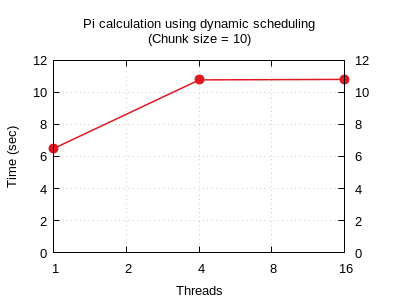
\includegraphics[width=0.55\columnwidth]{../ex1/plots/pi_c10.png}
  \caption{Timing results of $\pi$ calculation using chunk size = 10 iterations}
\end{figure}

%------------------------------------ 3

\begin{table}[htbp]
  \centering
    \begin{tabular}{|c c||l l l l| l|} 
    \hline
    \multicolumn{7}{|c|}{Timing results of $\pi$ calculation (Time unit: seconds)} \\
    \hline
    Chunk Size & \# of threads & 1st run & 2nd run & 3rd run & 4thr run & Average time\\ [0.5ex] 
    \hline\hline
    100 & 1 & 6.275921 & 6.279012 & 7.893470 & 6.281098 & 6.68237525 \\
    \hline
    100 & 4 & 2.428611 & 2.464799 & 2.463414 & 2.425332 & 2.445539 \\
    \hline
    100 & 16 & 2.425184 & 2.459710 & 2.432488 & 2.458897 & 2.44406975 \\ [1ex]
    \hline
    \end{tabular}
  \caption{Timing results of $\pi$ calculation using chunk size = 100 iteration}
\end{table}

\begin{figure}[htbp]
  \centering
  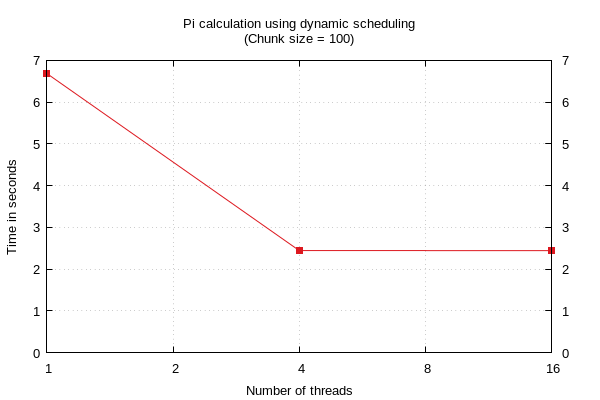
\includegraphics[width=0.55\columnwidth]{../ex1/plots/pi_c100.png}
  \caption{Timing results of $\pi$ calculation using chunk size = 100 iterations}
\end{figure}

%------------------------------------ 4

\begin{table}[htbp]
  \centering
    \begin{tabular}{|c c||l l l l| l|} 
    \hline
    \multicolumn{7}{|c|}{Timing results of $\pi$ calculation (Time unit: seconds)} \\
    \hline
    Chunk Size & \# of threads & 1st run & 2nd run & 3rd run & 4thr run & Average time\\ [0.5ex] 
    \hline\hline
    1000 & 1 & 6.248489 & 6.254362 & 6.254913 & 6.251492 & 6.252314 \\
    \hline
    1000 & 4 & 1.733363 & 1.735331 & 1.732440 & 1.734742 & 1.733969 \\
    \hline
    1000 & 16 & 1.731060 & 1.726669 & 1.730891 & 1.732937 & 1.73038925 \\ [1ex]
    \hline
    \end{tabular}
  \caption{Timing results of $\pi$ calculation using chunk size = 1000 iteration}
\end{table}

\begin{figure}[htbp]
  \centering
  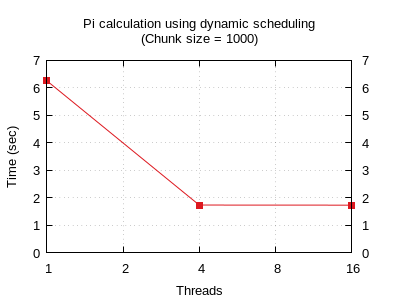
\includegraphics[width=0.55\columnwidth]{../ex1/plots/pi_c1000.png}
  \caption{Timing results of $\pi$ calculation using chunk size = 1000 iterations}
\end{figure}

%------------------------------------ 5


\begin{table}[htbp]
  \centering
    \begin{tabular}{|c c||l l l l| l|} 
    \hline
    \multicolumn{7}{|c|}{Timing results of $\pi$ calculation (Time unit: seconds)} \\
    \hline
    Chunk Size & \# of threads & 1st run & 2nd run & 3rd run & 4thr run & Average time\\ [0.5ex] 
    \hline\hline
    10000 & 1 & 6.244337 & 6.252478 & 6.250002 & 6.252064 & 6.24972025 \\
    \hline
    10000 & 4 & 1.664214 & 1.659239 & 1.660260 & 1.659163 & 1.660719 \\
    \hline
    10000 & 16 & 1.660762 & 1.664066 & 1.661164 & 1.658869 & 1.66121525 \\ [1ex]
    \hline
    \end{tabular}
  \caption{Timing results of $\pi$ calculation using chunk size = 10000 iteration}
\end{table}

\begin{figure}[htbp]
  \centering
  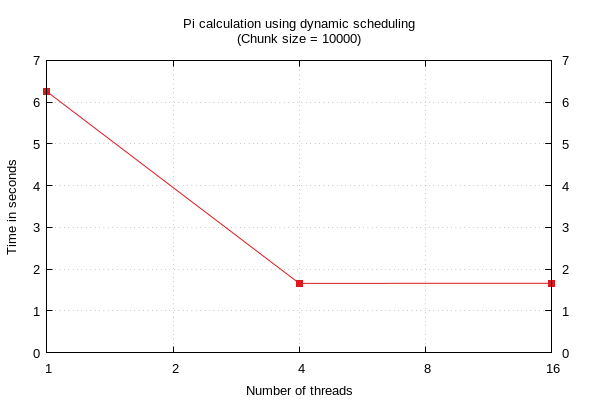
\includegraphics[width=0.55\columnwidth]{../ex1/plots/pi_c10000.png}
  \caption{Timing results of $\pi$ calculation using chunk size = 10000 iterations}
\end{figure}

%------------------------------------ 6


\begin{table}[htbp]
  \centering
    \begin{tabular}{|c c||l l l l| l|} 
    \hline
    \multicolumn{7}{|c|}{Timing results of $\pi$ calculation (Time unit: seconds)} \\
    \hline
    Chunk Size & \# of threads & 1st run & 2nd run & 3rd run & 4thr run & Average time\\ [0.5ex] 
    \hline\hline
    100000 & 1 & 6.237799 & 6.234975 & 6.244593 & 6.235083 & 6.2381125 \\
    \hline
    100000 & 4 & 1.661888 & 1.658459 & 1.667569 & 1.651900 & 1.659954 \\
    \hline
    100000 & 16 & 1.653965 & 1.652250 & 1.651300 & 1.651015 & 1.6521325 \\ [1ex]
    \hline
    \end{tabular}
  \caption{Timing results of $\pi$ calculation using chunk size = 100000 iteration}
\end{table}

\begin{figure}[htbp]
  \centering
  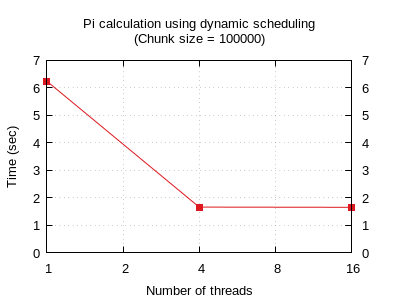
\includegraphics[width=0.55\columnwidth]{../ex1/plots/pi_c100000.png}
  \caption{Timing results of $\pi$ calculation using chunk size = 100000 iterations}
\end{figure}

%------------------------------------
\pagebreak

\subsection{Conclusion}
Based on the results presented above and given that the average execution time of the serial
program is 6,245896 seconds, we conclude that:

\begin{itemize}
 \item Program performance is increased until oversubscription appears. Even though we expect
       overheads to be introduced due to time slicing (e.g. context switching, cache pollution),
       the execution time becomes approximately constant after the number of threads exceeds
       the number of the processors available (4). This happens because switching between
       threads is less resource-intensive than switching between processes.
 \item Self-scheduling leads to execution times multiple times greater than the one of the
       serial program and in case of multithreaded calculation, dozens of times greater.
       The chunk size of one (1) iteration is a fine-grained task something that results
       in threads constantly racing to acquire the same mutex lock. As the number of threads
       is increased, race overhead is increased too. Moreover, the granularity of self-scheduling
       leads to more function calls taking place, something that adds up to the existing overheads.
 \item A single thread executing tasks with chunk size $\geq$ 10 requires almost the same time
       as the serial program.
 \item Multiple threads and tasks with chunk size $\ll 10^2$ result in higher execution times
       compared to the serial program. The reasons for these overheads are the same as in
       self-scheduling (fine-grained parallelism).
 \item Parallel program efficiency is unfolded for chunk size $\geq 10^2$ but hits a bottleneck
       for more coarse-grained tasks (chunk size $\geq 10^4$ iterations in this case).
\end{itemize}





\end{document}